%% This is file `elsarticle-template-1-num.tex',
%%
%% Copyright 2009 Elsevier Ltd
%%
%% This file is part of the 'Elsarticle Bundle'.
%% ---------------------------------------------
%%
%% It may be distributed under the conditions of the LaTeX Project Public
%% License, either version 1.2 of this license or (at your option) any
%% later version.  The latest version of this license is in
%%    http://www.latex-project.org/lppl.txt
%% and version 1.2 or later is part of all distributions of LaTeX
%% version 1999/12/01 or later.
%%
%% Template article for Elsevier's document class `elsarticle'
%% with numbered style bibliographic references
%%
%% $Id: elsarticle-template-1-num.tex 149 2009-10-08 05:01:15Z rishi $
%% $URL: http://lenova.river-valley.com/svn/elsbst/trunk/elsarticle-template-1-num.tex $
%%
\documentclass[preprint,12pt]{elsarticle}

%% Use the option review to obtain double line spacing
%% \documentclass[preprint,review,12pt]{elsarticle}

%% Use the options 1p,twocolumn; 3p; 3p,twocolumn; 5p; or 5p,twocolumn
%% for a journal layout:
%% \documentclass[final,1p,times]{elsarticle}
%% \documentclass[final,1p,times,twocolumn]{elsarticle}
%% \documentclass[final,3p,times]{elsarticle}
%% \documentclass[final,3p,times,twocolumn]{elsarticle}
%% \documentclass[final,5p,times]{elsarticle}
%% \documentclass[final,5p,times,twocolumn]{elsarticle}

%% The graphicx package provides the includegraphics command.
\usepackage{graphicx}
%% The amssymb package provides various useful mathematical symbols
\usepackage{amssymb}
%% The amsthm package provides extended theorem environments
%% \usepackage{amsthm}

%% The lineno packages adds line numbers. Start line numbering with
%% \begin{linenumbers}, end it with \end{linenumbers}. Or switch it on
%% for the whole article with \linenumbers after \end{frontmatter}.
\usepackage{lineno}

\usepackage{hyperref}
\usepackage{enumitem}
\usepackage[utf8]{inputenc}
\usepackage[T1]{fontenc}
\usepackage{minted}
\definecolor{bg}{rgb}{0.95,0.95,0.95}

%% natbib.sty is loaded by default. However, natbib options can be
%% provided with \biboptions{...} command. Following options are
%% valid:

%%   round  -  round parentheses are used (default)
%%   square -  square brackets are used   [option]
%%   curly  -  curly braces are used      {option}
%%   angle  -  angle brackets are used    <option>
%%   semicolon  -  multiple citations separated by semi-colon
%%   colon  - same as semicolon, an earlier confusion
%%   comma  -  separated by comma
%%   numbers-  selects numerical citations
%%   super  -  numerical citations as superscripts
%%   sort   -  sorts multiple citations according to order in ref. list
%%   sort&compress   -  like sort, but also compresses numerical citations
%%   compress - compresses without sorting
%%
%% \biboptions{comma,round}

% \biboptions{}

\journal{NeuroImage}

\begin{document}

\begin{frontmatter}

%% Title, authors and addresses

\title{The Brainomics/Localizer database}

%% use the tnoteref command within \title for footnotes;
%% use the tnotetext command for the associated footnote;
%% use the fnref command within \author or \address for footnotes;
%% use the fntext command for the associated footnote;
%% use the corref command within \author for corresponding author footnotes;
%% use the cortext command for the associated footnote;
%% use the ead command for the email address,
%% and the form \ead[url] for the home page:
%%
%% \title{Title\tnoteref{label1}}
%% \tnotetext[label1]{}
%% \author{Name\corref{cor1}\fnref{label2}}
%% \ead{email address}
%% \ead[url]{home page}
%% \fntext[label2]{}
%% \cortext[cor1]{}
%% \address{Address\fnref{label3}}
%% \fntext[label3]{}


%% use optional labels to link authors explicitly to addresses:
%% \author[label1,label2]{<author name>}
%% \address[label1]{<address>}
%% \address[label2]{<address>}

\author[Neurospin]{Dimitri Papadopoulos Orfanos\corref{mycorrespondingauthor}}
\ead{dimitri.papadopoulos@cea.fr}
\cortext[mycorrespondingauthor]{Corresponding author}
\author[Logilab]{Vincent Michel}
\author[Parietal,Neurospin]{Yannick Schwartz}
\author[U992,Neurospin,ParisSud]{Philippe Pinel}
\author[U992,Neurospin,ParisSud]{Antonio Moreno}
\author[Neurospin]{Denis Le Bihan}
\author[Neurospin]{Vincent Frouin}

\address[Neurospin]{CEA, DSV/I2BM, NeuroSpin, 91191 Gif-sur-Yvette, France}
\address[U992]{INSERM, U992, Cognitive Neuroimaging Unit, 91191 Gif-sur-Yvette, France}
\address[Parietal]{Parietal team, Inria Saclay \^Ile-de-France, 91120 Palaiseau, France}
\address[ParisSud]{Univ. Paris-Sud, Cognitive Neuroimaging Unit, 91191 Gif-sur-Yvette, France}
\address[Logilab]{Logilab, 104 boulevard Auguste Blanqui, 75013 Paris, France}

\begin{abstract}
%% Text of abstract
The Brainomics/Localizer database exposes part of the data collected by the in house Localizer project, which planned to acquire four types of data from volunteer research subjects: anatomical MRI scans, functional MRI data, behavioral and demographic data, and DNA sampling. Over the years, this local project has been collecting such data from hundreds of subjects. We had selected 94 of these subjects for their complete datasets, including all four types of data, as the basis for a prior publication; the Brainomics/Localizer database publishes the data associated to these 94 subjects. Since regulatory rules prevent us from making genetics data available for download, the database serves only anatomical MRI scans, functional MRI data, behavioral and demographic data.

To publish this set of heterogeneous data, we use dedicated software based on the open-source CubicWeb semantic web framework. Through genericity in the data model and flexibility in the display of data (web pages, CSV, JSON, XML), CubicWeb helps us expose these complex datasets in original and efficient ways.
\end{abstract}

\begin{keyword}
%********** Science \sep Publication \sep Complicated
%% keywords here, in the form: keyword \sep keyword

%% MSC codes here, in the form: \MSC code \sep code
%% or \MSC[2008] code \sep code (2000 is the default)

imaging genetics \sep database \sep semantic web
\end{keyword}

\end{frontmatter}

%%
%% Start line numbering here if you want
%%
%********** \linenumbers

%% main text
\section{Introduction}

The Brainomics/Localizer database is a data repository containing datasets from 94 subjects with structural MRI scans, functional MRI data, behavioral and demographics data. DNA sampling has been performed on the subjects, but we cannot publish such data due to regulatory rules.

Datasets have been acquired by the in house Localizer project which initially planned to investigate inter-subject variability \cite{Pinel2007}. We have been collecting data from volunteer research subjects taking part in different studies carried out in our lab. The investigators of these studies agreed to provide behavioral and demographic data, anatomical MRI scans and DNA sampling. They also agreed to acquire a short fMRI sequence, approximatively 5 minutes long, after their functional imaging session, specifically for the Localizer project. We were thus able to collect data from a considerably larger number of volunteer research subjects than a single study could afford.

We have also been working on genetic neuroimaging in the context of the Brainomics project. We felt the need for a database that could index and expose heterogeneous data including MRI images, genetic data or behavioral data. We based our software developments on the CubicWeb semantic web framework and wrote specific CubicWeb modules to describe and visualize neuroimaging and genetic data. We decided to build a Brainomics/Localizer demonstrator based on the Localizer dataset. The resulting database is now publicly available\footnote{\url{http://brainomics.cea.fr/localizer}} as well as the source code\footnote{\url{https://github.com/neurospin/localizer}}.

We also viewed the Brainomics/Localizer demonstrator as an opportunity to study the feasibility of opening up medical research data as support material for scientific articles. Regulatory rules differ from country to country and may hamper homogeneous publication of scientific data: we do not know of other public databases of research individual health information in France--and suspect there are very few.


\section{Material and methods}

\subsection{De-identification of the database}
\label{sec:de-identification}

The local ethics committee had initially approved the Localizer study. Starting the Brainomics/Localizer database effort, we addressed with the ethics committee the publication of Localizer data as support material for one of the published paper \cite{Pinel2012}, in order to facilitate replication of the results. The following paragraphs describe the agreement that led to the publication. Please note that not all described functionality has been implemented. More specifically we currently do not provide means to run calculations involving genetic data. As a result genetic information is currently not publicly available from the database, although it is internally available to the server.

\begin{quotation}
Before publishing the data, we anonymize it in an irreversible way by re-encoding all subject identifiers and discarding the conversion table. Data is stored on an online server and made available to the broader scientific community as a web service. Users can access the data from a web browser.
\end{quotation}
In our lab, any mention of name, social security number or other similar data are prohibited in all the data acquired for research purposes. Instead we use a subject identifier; the correspondence between this local identifier and sensitive data, such as names, is kept securely. Conversion methods are hosted on a specific system restricted to medical staff. The publication process requires that local identifiers are converted into new random identifiers and the conversion table is discarded.

As a result of this irreversible re-encoding, updates are not straightforward. In the event we have to remove a subject, we would have to get back to the source data on our internal network, remove data based on local subject identifiers and then re-encode them to new random identifiers.

\begin{quotation}
\textit{Imaging data} In addition to re-encoding subject identifiers, anatomical MRI images are defaced.
\end{quotation}
We used the \textit{mri\_deface} tool of Freesurfer \cite{Fischl2012} to deface anatomical images.

\begin{quotation}
\textit{Genetic data} The very nature of genotyping data strongly identifies a subject, by mere comparison to other genotyping data collected elsewhere. As a result genetic data cannot be downloaded from the server. Users can nevertheless start calculations on the server itself from a user interface, using the genetic data of all subjects as a parameter. The results of such calculations are images like those presented in Fig.~1 of \cite{Pinel2012}. These actions should be crafted carefully to forbid retrieval of individual genotypic data.

\textit{Demographic and behavioral data} Only data related to the publication \cite{Pinel2007} are uploaded to the server. Such data do not present a risk of identifying the subject.
\end{quotation}
We feel it is hard to identify an individual by comparing the demographics and behavioral data available from the database to similar data collected elsewhere. Contrarily DNA samples collected elsewhere could easily be compared and matched with DNA data from the database.

\subsection{Software infrastructure}

\subsubsection{The Brainomics genetic neuroimaging database}

The need to manage data growing in volume and complexity have led the neuroimaging field to rely increasingly on database infrastructures. These databases typically provide support for multiple data types \textit{e.g.}, brain images, behavioral and demographic data, neuropsychological scores, and genetic data. Popular solutions for storing such data at a large scale are COINS \cite{COINS2011} and XNAT \cite{XNAT2007}. 

We chose CubicWeb\footnote{\url{https://www.cubicweb.org}}, which is an alternative open-source framework. We customized it for the requirements of imaging genetics. The resulting Brainomics genetic neuroimaging database permits deep integration of imaging and genetic data \cite{HBM2013}. We use it internally to query jointly genetic and neuroimaging data--but as already explained the publicly available database currently excludes genetic data.

XNAT and COINS not only expose neuroimaging data, they also collect and even process data. In contrast we focused on exposing and offering different views on the data, including web pages for human consumption, mechanisms for download, and semantic-web queries run from processing software.

\subsubsection{The CubicWeb framework}
\label{sec:cubicweb}

The CubicWeb framework follows the semantic web approach: data are exposed using ontologies for easier sharing, access, and processing, and each item is identified by a unique ID (called \textit{Uniform Resource Identifier} or URI). CubicWeb is built upon well established core technologies such as SQL, Python and web standards (HTML5 and JavaScript). It has been successfully used in large semantic web and knowledge management projects \cite{Simon2013}.

One major part of a CubicWeb application is the data model, defined as \textit{entities} and \textit{relations} by Python classes, from which CubicWeb generates the underlying SQL tables. It is thus possible to query the data via the RQL language which predates but is similar to W3C's SPARQL. This language provides an abstraction over the underlying database, queries being expressed in terms of business logic rather than low-level SQL schema. For example, \emph{Query all the scans of male subjects} can be expressed in RQL as \emph{Any X WHERE S is Subject, S gender "male", X is Scan, X concerns S}.

Moreover, CubicWeb implements a mechanism to expose information in several ways called \emph{views}. Being defined in Python, the views are applied on query results, and can produce any kind of output, such as web pages, but also binary data or even trigger external processing. The separation of queries and views holds major advantages:
\begin{enumerate}[label=\roman*)]
\item The same data selection may have several representations, \textit{e.g.} the subject \emph{S65}, defined by a single query (\textit{Any X WHERE X is Subject, X identifier "S65"}) can be viewed as HTML, or downloaded in the JSON, RDF or CSV formats (see Listing~\ref{code:rql}). Each couple \textit{(query, view)} is identified by a unique Universal Resource Locator (URL).
\item Data can be exported in several other formats (\textit{e.g.} XCEDE or MAGE-ML interchange formats) without modifying the underlying data storage. The data model can be performance-oriented, adding a new ontology for sharing the data being simply a new view to define.
\end{enumerate}

\begin{listing}[H]
\begin{minted}[bgcolor=bg, fontsize=\scriptsize]{text}
http://brainomics.cea.fr/localizer/dataset?rql=Any X WHERE X is Subject, X identifier "S65"
http://brainomics.cea.fr/localizer/dataset?rql=Any X WHERE X is Subject&vid=csvexport
http://brainomics.cea.fr/localizer/dataset?rql=Any X WHERE X is Subject&vid=xcede
\end{minted}
\caption{Example of URLs containing RQL queries. They permit to uniquely identify data associated with the queries in the Localizer database. From top to bottom: select subject "S65" and by default display a web page, select all subjects and return the results as a CSV tabular file, and select all subjects and return the results in the XCEDE format.}
\label{code:rql}
\end{listing}

Finally, CubicWeb has a security system, coupled to the data model definition, that grants fine-grained data access rights. CubicWeb may run as a standalone application or use Apache as a front end and an alternative for logging, monitoring or authentication purposes. CubicWeb may also use LDAP as an alternate source for user credentials and information.

\subsubsection{Development of domain specific modules}

We developed one \textit{cube} (CubicWeb module) per data type. Each cube is connected to the others -- if needed -- in the final database schema. The \textit{medicalexp} cube contains the definition of general \textit{entities} (or classes of objects) like Subject, Center, Assessment; the \textit{neuroimaging} (resp. \textit{genetics}) cube defines entities and relations like Scan, Scanner (resp. SnpVariant, Platform, GenotypeMeasurement). The concepts have been be modeled as much as possible upon the XCEDE \cite{keator2006general} schema. Each cube implements the corresponding views (navigation, download), triggers and access rights. Connected together, those cubes and others are used to build the complete Brainomics/Localizer database (Fig.~\ref{fig:ui}). Like the CubicWeb framework, these cubes are distributed under the LGPL license and the source code is available from the CubicWeb web site\footnote{\url{https://www.cubicweb.org/project/cubicweb-brainomics}}.

\begin{figure}[ht!]
    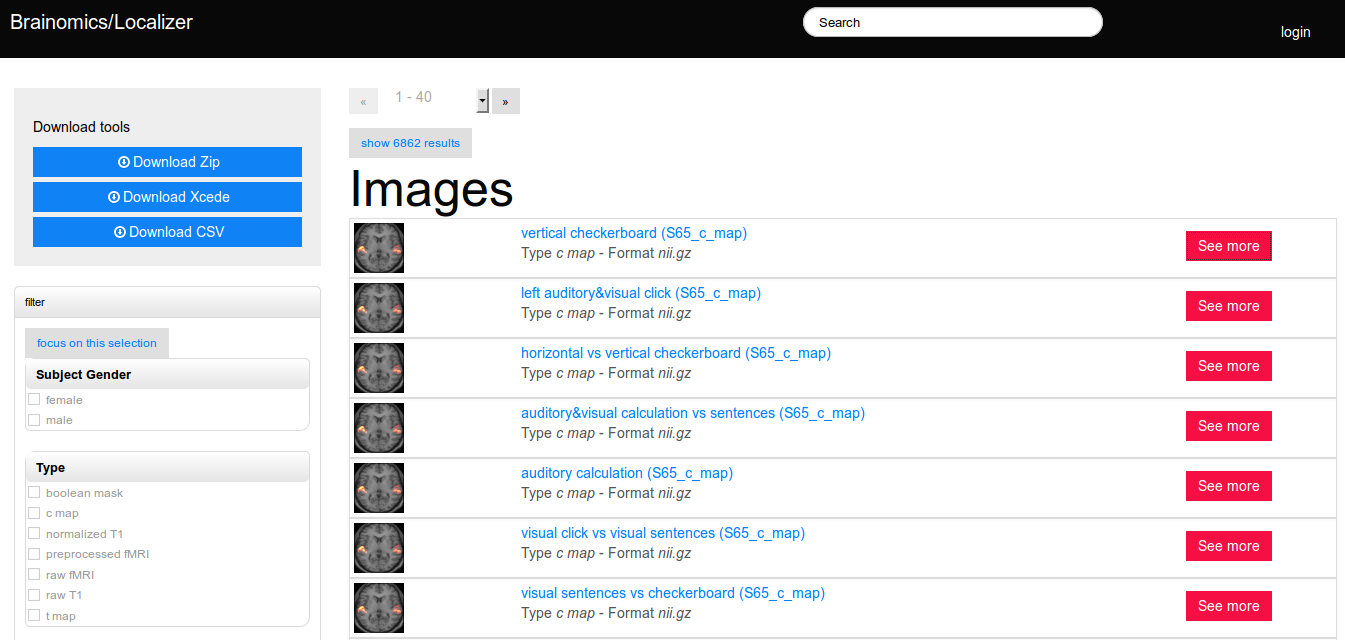
\includegraphics[width=\textwidth]{ui1}
    \caption{Screenshot of the Brainomics web interface, showing the downloading and filtering \emph{facets} (menus) on the left, and the summary representation of the images stored in the database.}
    \label{fig:ui}
\end{figure}

These domain specific modules add the capacity to download data in the XCEDE \cite{keator2006general} format, in addition to the JSON, RDF and CSV formats natively supported by CubicWeb.


\section{Description of the repository}

\subsection{Purpose of the database}

Our database was designed to publish data from the Localizer project \cite{Pinel2007} and more specifically the subset of 94 subjects examined in \cite{Pinel2012}, and make it available to the broader scientific community. Our intent was to set up a demonstrator for the software we have developed in the context of our Brainomics project.

We provide a static set of data. In the short term we have no plans for adding data from other subjects of the Localizer study.

\subsection{Available data}

Of the hundreds of subjects acquired in house by the Localizer project, we selected a subset of 94 subjects for their complete datasets \cite{Pinel2012} including anatomical MRI scans, functional MRI data, behavioral and demographic data, and DNA sampling. Retained subjects were mostly young Caucasian highly educated, mostly normal readers, 49 women and 45 men. The exact age of 4 subjects remains unknown, the rest were from 18 through 49 years old -- mean age was 24.7 years old. All subjects were right-handed and native French speakers.

Demographic data displayed by the database include gender, age at the time of inclusion, handedness, native language and a family identifier which helps identifying siblings.

Behavioral data aimed to create a rough cognitive profile of each subject. Each profile contains scores for 126 questions covering education, developmental disorders, reading difficulties, basic numerical knowledge, arithmetical skills, visuo-spatial abilities, and visuo-motor abilities.

Two 3~T MRI scanners have been used by our lab for routine acquisitions over time, a Bruker 3~T scanner and a Siemens Trio Tim 3~T scanner. The MRI data were acquired on either of these scanners. 

Data processing was performed with SPM8 \footnote{\url{http://www.fil.ion.ucl.ac.uk/spm/software/spm8/}}. The anatomical scan was spatially normalized to the ICBM152 T1-weighted brain template defined by the Montreal Neurological Institute using the default parameters (including the nonlinear transformations and trilinear interpolation). Raw and processed MRI data are available in the NIfTI format. Both raw and normalized T1-weighted anatomical MRI scans are provided for each subject. Functional MRI data includes raw EPI scans, preprocessed fMRI scans and statistical parametric maps. The fMRI experimental design as well as data processing are described in more detail in the initial Localizer article \cite{Pinel2007}. Let us only cite the challenging constraints taken into account when designing the sequence:
\begin{itemize}
\item the sequence had to be short, so as to disrupt as little as possible the main protocol. We choose 5 minutes for performing 100 trials.
\item we aimed to obtain for each subject a description of different levels of functional architecture, from sensorimotor areas (perception and action) to more associative areas involved in reading, language processing and calculation.
\item we aimed to capture in 5 minutes most of the individual networks related to each task.
\item individual networks described in 5~min had to be reproducible over sessions and time.
\end{itemize}

Images are made available as NIfTI files. They can be downloaded as ZIP files from the Brainomics/Localizer server. Other data can be viewed in tabular form in the Web interface and exported to a variety of formats such as JSON, RDF, CSV and XCEDE, as described in paragraph~\ref{sec:cubicweb}.

A URI is associated to every entity stored in the database, such as a Subject, a Scan or a ScanGenotypeMeasurement. Furthermore, a URI is also associated to every \emph{(query, view)} couple used to select and display or download data. Such URIs can be kept as a permanent link to complex sets of data.

\begin{listing}[H]
\begin{minted}[linenos=true, bgcolor=bg, fontsize=\scriptsize]{python}
import numpy as np

from sklearn.cross_validation import LeaveOneLabelOut, cross_val_score
from sklearn.linear_model import LogisticRegression
from nilearn.datasets import fetch_localizer_contrasts
from nilearn.input_data import NiftiMasker

# fetch the specified tasks from the localizer database

tasks = [
    'horizontal checkerboard',
    'vertical checkerboard',
    'sentence reading',
    'calculation (auditory cue)',
    'calculation (visual cue)',
    'left button press (auditory cue)',
    'left button press (visual cue)',
    'right button press (auditory cue)',
    'right button press (visual cue)',
]

localizer_data = fetch_localizer_contrasts(tasks, get_tmaps=True)
images = np.array(localizer_data['tmaps'])

# we denote the statistical maps as X, and the target to predict as y
masker = NiftiMasker(standardize=True, memory='cache')
X = masker.fit_transform(images)
y = np.array(['calc' if 'calculation' in img else 'non-calc' for img in images])

# we perform a leave-one subject out cross validation
cv = LeaveOneLabelOut(ext_vars.subject_id.values)

# we use a LogisticRegression classifier with default parameters
clf = LogisticRegression()

scores = cross_val_score(clf, X, y, cv=cv, n_jobs=-1, verbose=1)
print 'scores mean=%.02f, std=%.02f' % (np.mean(scores), np.std(scores))
\end{minted}
\caption{Example of NiLearn's Localizer fetcher: the Localizer database data are directly downloaded from Python code and used to learn a model that predicts calculation tasks.}
\label{code:NiLearn}
\end{listing}

\subsection{Quality control and review of the data}

All anatomical MRI scans have been examined by radiologists for possible health issues. A \emph{summary sheet} (Fig.~\ref{fig:summary}) was generated for every subject to evaluate the quality of the fMRI acquisition. A script based on SPM scripts generates movement curves or \textit{glass brain}. For each contrast a specific region of interest (ROI) has been defined. For each subject, the quality of a contrast is evaluated as the ratio of activated voxels in the ROI to the mean number of voxels activated in the ROI across all 94 subjects. Good contrasts are defined by a ratio of over 10\%. We checked the summary sheets one by one and all 94 selected subjects were considered good enough with scores of 5 or 6 good contrasts out of 6.

\begin{figure}[ht!]
    \centering
    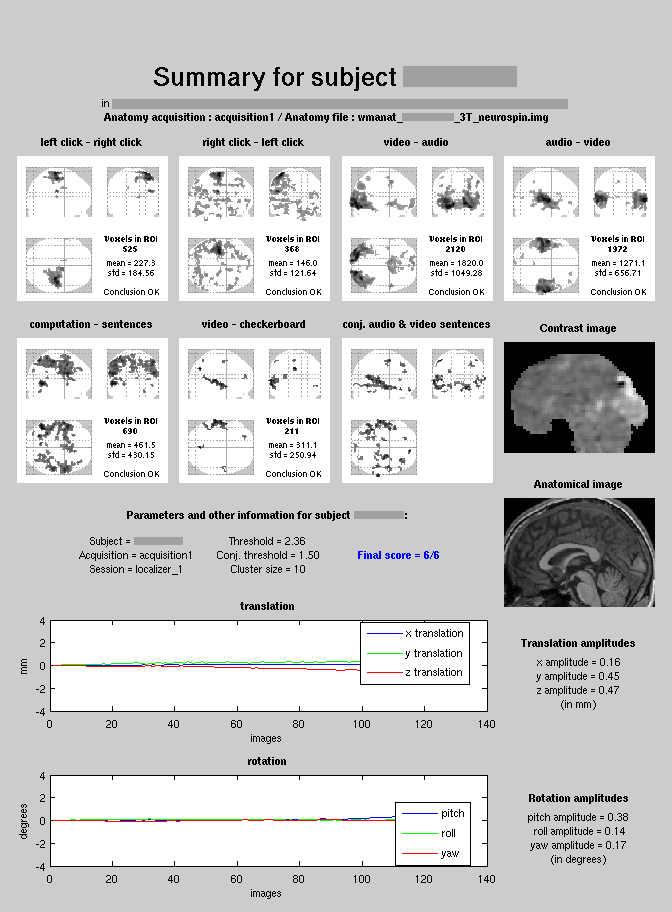
\includegraphics[scale=0.4]{summary}
    \caption{This summary sheet generated for each of the subjects helps assess the quality of the fMRI acquisition. The summary sheet shows, in the lower half, the translation and rotation movement curves for the subject, with maximal amplitudes printed beside the graphics. It also shows sagittal views of the normalized anatomy and of an unthresholded contrast in order to check that normalization has been performed correctly. In the upper half of the sheet, six selected contrasts and a conjunction of two contrasts are shown on \emph{glass brain} figures. The goal of these images is to verify that the main activations are in the expected regions of the brain. This is done visually but also a quick test is performed: for each contrast, regions of interest and adapted thresholds are defined and, if the activation for the subject is good enough, the contrast is considered correct. Therefore, if the six contrasts are good, the \emph{final score} that appears in the middle part of the sheet will be equal to 6. If only two of them are correct, the score will be 2/6. Other processing parameters are also shown in the middle and top of this summary sheet.}
    \label{fig:summary}
\end{figure}

Demographic data were obtained from different sources, questionnaires performed by the nurses and other questionnaires by the experimenters. We cross-checked redundant information and looked for suspect values wherever possible while merging information from these different sources.

We manually reviewed behavioral data for each subject in the same way, checking that the relevant tables in the database matched correctly the paper questionnaires from which they were extracted.

DNA sample processing was outsourced to a specialized lab. Genetics data were roughly controlled by us too, mainly in order to include them in the proper format.

\subsection{How to access the data}

Data are available to everyone, without prior authentication, at \url{http://brainomics.cea.fr/localizer}. A registration process had initially been set up but later removed because it deterred users from trying to access the data. The same mechanism is used for imaging and phenotypic data. Imaging data can be selected in the web user interface, and then packed into a ZIP file that can be downloaded. Phenotypic data are directly available in tabular form in the web user interface and can be downloaded as a CSV file among other formats.

Data are made available under the Creative Commons 3.0 licence (CC BY 3.0). We ask our work is acknowledged in publications that use data from the Brainomics/Localizer database. Thanks to the permissive license, the statistical parametric maps are also downloadable from NeuroVault \cite{NeuroVault2014}, as we aim to make the Localizer data available to a broader audience.
The fMRI data can be downloaded from the NiLearn Python library \cite{NiLearn} as an example dataset, which may be used as a testbed to gauge analytic techniques.

\subsection{Data updates}

Users do not authenticate on our server. We therefore have no way of updating them other than posting information on the web site.

Since this database comes in support of an existing publication \cite{Pinel2012}, we do not plan on adding new subjects or modifying existing subjects. In the event of subject withdrawal, as explained in paragraph \ref{sec:de-identification}, regulatory rules leave us no choice but using new random identifiers for all subjects. The only option in that case would be to inform of a removal, without being able to identify the removed subject.

\subsection{Future developments}

The current file download architecture is similar to the one found in XNAT: a ZIP file is created containing the files associated to a specific query and can then be downloaded. We plan on developing a faster and more robust process, providing persistent links to the files associated to the result of a query.

Although we do not plan on hosting new data in this specific database, we do operate other databases running the same CubicWeb/Brainomics software, for projects such as IMAGEN \cite{Imagen2010} or EU-AIMS \cite{Aims2014} which keep collecting and exposing new data.

The long term plans for this resource is to keep it alive as a public example instance of our software. Since the data itself is mostly frozen, the database can be seen as a ``technical object'' that can be handed over to the team of engineers and IT specialists who will be managing the other databases based on the same software.


\section{Conclusion}

We opened up heterogeneous data from 94 subjects of the Localizer project, selected for the completeness of available data including anatomical MRI scans, functional MRI data, behavioral and demographic data. DNA sampling cannot be made publicly available due to regulatory rules. The 94 datasets can be downloaded under a permissive license.

The data are made available on a dedicated server hosting the Brainomics/Localizer database. The database is built upon the CubicWeb semantic web framework and a few extension modules that define the data model and \emph{views}. It supports standard metadata formats in neuroimaging such as XCEDE and defines permanent URLs for each queryable entity in the database.


\section{Acknowledgements}

This work was supported by ANR-10-BINF-04. We thank Stanislas Dehaene for his participation to the creation and for the sharing of the Localizer database. We thank the Inria-CEA Parietal team and in particular Virgile Fritsch for the Localizer data fetcher in NiLearn.

%% The Appendices part is started with the command \appendix;
%% appendix sections are then done as normal sections
%% \appendix

%% \section{}
%% \label{}

%% References
%%
%% Following citation commands can be used in the body text:
%% Usage of \cite is as follows:
%%   \cite{key}          ==>>  [#]
%%   \cite[chap. 2]{key} ==>>  [#, chap. 2]
%%   \citet{key}         ==>>  Author [#]

%% References with bibTeX database:

\bibliographystyle{elsarticle-num}

\bibliography{brainomics_localizer.bib}

%% Authors are advised to submit their bibtex database files. They are
%% requested to list a bibtex style file in the manuscript if they do
%% not want to use model1-num-names.bst.

%% References without bibTeX database:

% \begin{thebibliography}{00}

%% \bibitem must have the following form:
%%   \bibitem{key}...
%%

% \bibitem{}

% \end{thebibliography}


\end{document}
